Como se dijo en la etapa de descompilado, Waze utiliza direcciones únicas para sus consultas y esta dirección puede ser utilizada por otras aplicaciones para ejecutar Waze con algún comando.
\\\\
Analizando los ejemplos para desarrolladores, una forma de invocar Waze es con la dirección “waze://q=” y concatenando la búsqueda y esto genera una búsqueda dentro de Waze tal como si el usuario la buscara.
\\\\
Por tanto, se probó en un sitio HTML que invocara la url “waze://q=Facultad de Ingeniería UDP, Chile Santiago” (http://output.jsbin.com/telecozazi) para que ejecutara Waze con esa búsqueda.

        \begin{figure}[H]
  \begin{center}
    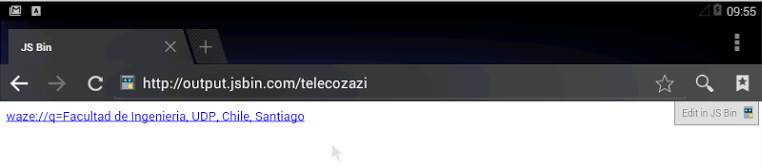
\includegraphics[width=0.3\textwidth]{imagenes/fig43.png}
    \caption{Sitio HTML que invoca url waze://}
  \end{center}
\end{figure}


Al abrir el enlace en el navegador de Android se ejecutó Waze generando la búsqueda dicha.

        \begin{figure}[H]
  \begin{center}
    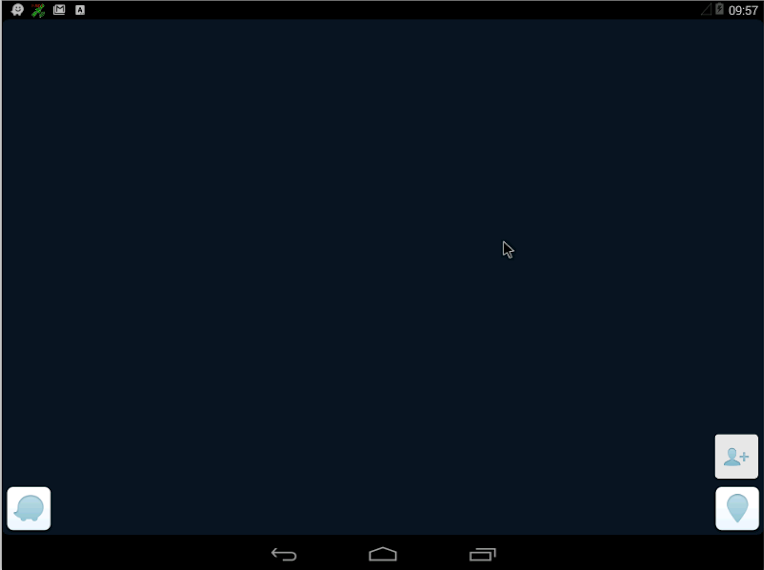
\includegraphics[width=0.3\textwidth]{imagenes/fig44.png}
    \caption{Ejecución de Waze al abrir la url Waze:// en la imagen anterior}
  \end{center}
\end{figure}


El mapa, no se muestra debido a que Waze de alguna manera detecta los programas que establecen ubicaciones que no corresponden, pero si realizó la acción solicitada.
